%Marco Teórico
\section{Marco Teórico}

    \subsection{Amplificador Operacional}

        Es técnicamente un amplificador electrónico, el cual activa su funcionamiento con corriente continua. Contiene una conexión de salida y dos conexiones de entrada. También, se identifica a estos dispositivos con las siglas OPAMP, tomado del término en inglés “operational amplifier”. El diferencial de potencia de ambas entradas es considerablemente menor comparado con el de la salida. 
        
        El amplificador está conformado por los siguientes parámetros:

        \begin{itemize}
            \item \textbf{Impedancia de entrada}

                Es la resistencia entre las entradas del amplificador.

            \item \textbf{Impedancia de salida}

                Es la resistencia que se observa a la salida del amplificador.

            \item \textbf{Ganancia en lazo abierto}
                Indica la ganancia de tensión en ausencia de realimentación. Se puede expresar en unidades naturales $(V/V \, \text{,} \, V/mV)$ o logarítmicas (dB).

            \item \textbf{Tensión en modo común}

                Comprende el valor promedio de tensión aplicada a ambas entradas del amplificador operacional.

            \item \textbf{Tensión offset}

                 El voltaje de desvió de entrada, también conocido como tensión de offset, es una pequeña tensión continua presente en la entrada de un amplificador operacional cuando no hay señal de entrada aplicada. Esta tensión puede alterar el comportamiento del amplificador operacional y afectar la precisión de la señal de salida en aplicaciones de alta precisión.

            \item \textbf{Corriente offset}

                Se trata de la diferencia de corriente entre las dos entradas del amplificador operacional, que hace que su salida tome el valor cero.

            \item \textbf{Tensión de entrada diferencial}

                Es la mayor diferencia de tensión entre las entradas del operacional que mantienen el dispositivo dentro de las especificaciones.

            \item \textbf{Corriente de polarización}

                Corriente media que circula por las entradas del operacional en ausencia de señal.

            \item \textbf{Slew rate o Tasa de variación de tensión}

                Es la máxima variación de la tensión de salida con respecto a la variación del tiempo, como respuesta a una tensión de escalón. 
                
                Se mide en $\dfrac{V}{\mu s}$, $\dfrac{kV}{\mu s}$ o unidades similares. Este parámetro está limitado por la compensación en frecuencia de la mayoría de los amplificadores operacionales.

            \item \textbf{Relación de Rechazo en Modo Común(CMRR)}

                Es la capacidad de un amplificador de rechazar señales en modo común.            
        \end{itemize}

    \subsection{Ganancia}

        La Ganancia es la proporción entre el nivel de salida y el nivel de entrada. La Ganancia entonces se expresa en "veces", lo que no tiene unidad; si la Ganancia expresa el nivel de salida respecto de un nivel específico referencia (que no tiene porqué ser la unidad de medida) entonces se dice que la Ganancia es de x veces sobre el valor de referencia.

        \begin{itemize}
            \item \textbf{Ganancia de Tensión}

                Si tratamos de tensión de salida de un amplificador, $V_{out}$, comparándola con la tensión de entrada, $V_{in}$, tendríamos la Ganancia en Tensión:

                \begin{gather}
                    A_v=\dfrac{V_{out}}{V_{in}}
                \end{gather}

            \item \textbf{Ganancia de intensidad}

                Si comparamos la intensidad de salida un amplificador, $I_{out}$, frente a la intensidad de entrada, $I_{in}$, tendríamos la Ganancia en Intensidad:

                \begin{gather}
                    A_I=\dfrac{I_{out}}{I_{in}}
                \end{gather}

            \item \textbf{Ganancia en potencia}

                Si comparamos la potencia de salida de salida, respecto de la potencia de entrada, lo que tendríamos sería la Ganancia en Potencia:

                \begin{gather}
                    A_P=\dfrac{P_{out}}{P_{in}}
                \end{gather}
        \end{itemize}

    \subsection{Topologías de los Amplificadores Operacionales}

        \subsubsection{Inversor}
        
            \begin{figure}[H]
              \centering              
              \includestandalone{Circuitos/inversor}
              \caption{Configuración del Amplificador Inversor}
              \label{fig:inversor0}
            \end{figure}
            
            Es un circuito electrónico que amplifica una señal de entrada aplicada a su entrada, produciendo una señal de salida que es inversa en fase a la señal de entrada. Es decir, si la señal de entrada aumenta, la señal de salida disminuirá y viceversa. Este tipo de amplificador se utiliza a menudo en aplicaciones de amplificación de señales de baja frecuencia, como en amplificadores de audio. 
            
            Su ganancia puede escribirse de la siguiente manera: 

            \begin{gather}
                A_v=\dfrac{V_{out}}{V_{in}}=\dfrac{R_6}{R_1}
            \end{gather}

        \subsubsection{No Inversor}

            \begin{figure}[H]
              \centering              \includestandalone{Circuitos/no_inversor}
              \caption{Configuración del Amplificador No Inversor}
              \label{fig:no_inversor0}
            \end{figure}

            Un amplificador no inversor es un tipo de amplificador electrónico en el cual la señal de salida es proporcional a la señal de entrada en fase, es decir, si la señal de entrada aumenta, la señal de salida también aumenta en la misma proporción. 
            
            Este tipo de amplificador se utiliza a menudo en aplicaciones de amplificación de señales de baja frecuencia, como en amplificadores de audio. En un amplificador no inversor, la señal de entrada se aplica a la entrada no inversora del amplificador operacional, mientras que la entrada inversora se conecta a un punto de referencia, generalmente a tierra. La ganancia de este tipo de amplificador se determina por la relación de resistencias en la configuración del circuito. 
            
            Su ganancia puede calcularse de la siguiente manera:

             \begin{gather}
                A_v=\dfrac{V_{out}}{V_{in}}=1+\dfrac{R_6}{R_1}
            \end{gather}

        \subsubsection{Integrador}

            \begin{figure}[H]
                \centering
                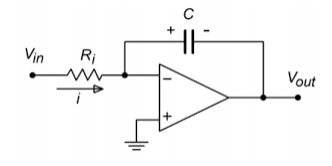
\includegraphics[width=8cm]{Imagenes/integrador.png}
                \caption{Configuración del Amplificador Integrador}
                \label{fig:integrador0}
            \end{figure}

             Un amplificador integrador es un circuito electrónico que realiza la operación matemática de integración en una señal de entrada. Es decir, la salida del amplificador integrador es proporcional a la integral de la señal de entrada. Este tipo de amplificador se utiliza a menudo en aplicaciones de procesamiento de señales, como en filtros pasa bajos. En un amplificador integrador, la señal de entrada se aplica a la entrada inversora del amplificador operacional, mientras que una resistencia y un capacitor se conectan en serie entre la entrada inversora y la salida del amplificador. La señal de salida es tomada en el capacitor, y la ganancia del circuito se determina por la relación entre la resistencia y la capacitancia en el circuito.
             
             Su ganancia puede calcularse de la siguiente manera:

             \begin{gather}
                  A_v=\dfrac{V_{out}}{V_{in}}=-\dfrac{1}{SCR_i}
             \end{gather}

        \subsubsection{Integrador de Boo (Integrador No Inversor}

            \begin{figure}[H]
              \centering              \includestandalone{Circuitos/integrador_no_inversor}
              \caption{Configuración del Integrador No Inversor}
              \label{fig:integrador_no_inversor0}
            \end{figure}

            La topología integrador no inversor, también conocida como integrador de Boo, es un circuito que utiliza un amplificador operacional para integrar una señal de entrada. A diferencia de un integrador inversor, en el que la entrada se aplica a través de una resistencia y la salida se toma directamente del capacitor, en un integrador no inversor la señal de entrada se aplica directamente al capacitor y la salida se toma a través de una resistencia conectada a la salida del amplificador operacional. El integrador no inversor se puede utilizar para una variedad de aplicaciones, como por ejemplo para la detección de cruce por cero, la medición de flujo, la regulación de voltaje y la eliminación de ruido en señales analógicas.

        \subsubsection{Derivador}

            \begin{figure}[H]
                \centering
                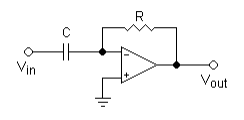
\includegraphics[width=8cm]{Imagenes/derivador.png}
                \caption{Configuración del Amplificador Derivador}
                \label{fig:derivador0}
            \end{figure}

            Un amplificador derivador es un circuito electrónico que realiza la operación matemática de derivación en una señal de entrada. Es decir, la salida del amplificador derivador es proporcional a la derivada de la señal de entrada. Este tipo de amplificador se utiliza a menudo en aplicaciones de procesamiento de señales, como en filtros pasa altos. En un amplificador derivador, la señal de entrada se aplica a la entrada inversora del amplificador operacional, mientras que una resistencia se conecta en serie entre la entrada inversora y la salida del amplificador. La señal de salida es tomada en la resistencia, y la ganancia del circuito se determina por la relación entre la resistencia y la capacitancia en el circuito. 
            
            
            Su ganancia puede calcularse de la siguiente manera:

            \begin{gather}
                  A_v=\dfrac{V_{out}}{V_{in}}=-SCR
             \end{gather}

        \subsubsection{Sumador Inversor}

            \begin{figure}[H]
                \centering
                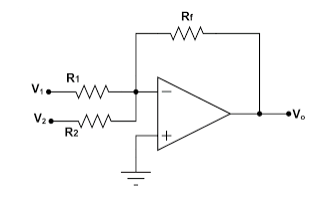
\includegraphics[width=8cm]{Imagenes/sumador_inversor.png}
                \caption{Configuración del Amplificador Sumador Inversor}
                \label{fig:sumador_inversor}
            \end{figure}

            Un amplificador sumador inversor es un circuito electrónico que suma varias señales de entrada y produce una señal de salida inversa en fase a la señal de salida de cada entrada. Este tipo de amplificador se utiliza a menudo en aplicaciones de procesamiento de señales, como en amplificadores de audio estéreo o en circuitos de mezcla de señales. En un amplificador sumador inversor, la señal de entrada se aplica a través de resistencias a las entradas inversoras del amplificador operacional. La señal de salida se toma en la salida del amplificador operacional, y la ganancia del circuito se determina por la relación entre las resistencias en el circuito. 
            
            Su ganancia puede calcularse de la siguiente manera: 

            \begin{gather}
                V_o=-R_f\left(\dfrac{V_1V_2}{R_1R_2}\right)
            \end{gather}

        \subsubsection{Restador}

            \begin{figure}[H]
              \centering              \includestandalone{Circuitos/restador}
              \caption{Configuración del Amplificador Restador}
              \label{fig:restador0}
            \end{figure}

            Un amplificador restador es un circuito electrónico que resta dos señales de entrada y produce una señal de salida que es proporcional a la diferencia entre ellas. Este tipo de amplificador se utiliza a menudo en aplicaciones de procesamiento de señales, como en circuitos de cancelación de ruido o en instrumentación de medición. En un amplificador restador, las dos señales de entrada se aplican a través de resistencias a las entradas inversoras del amplificador operacional. La señal de salida se toma en la salida del amplificador operacional, y la ganancia del circuito se determina por la relación entre las resistencias en el circuito. 
            
            Su ganancia puede calcularse de la siguiente manera: 

            \begin{gather}
                V_o=-\dfrac{R_6}{R_1}V_1+\dfrac{R_5}{R_5+R_3}V_3\left(1+\dfrac{R_6}{R_1}\right) 
            \end{gather}

        \subsubsection{Diferencial}

            \begin{figure}[H]
                \centering
                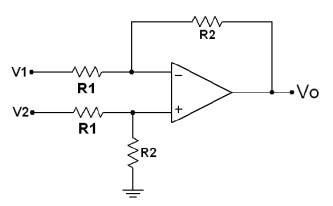
\includegraphics[width=8cm]{Imagenes/diferencial.png}
                \caption{Configuración del Amplificador Diferencial}
                \label{fig:diferencial0}
            \end{figure}

            Un amplificador diferencial es un circuito electrónico que amplifica la diferencia entre dos señales de entrada y produce una señal de salida proporcional a esta diferencia. Este tipo de amplificador se utiliza a menudo en aplicaciones de procesamiento de señales, como en amplificadores de instrumentación y en amplificadores de audio de alta calidad. En un amplificador diferencial, dos señales de entrada se aplican a las entradas inversoras y no inversoras del amplificador operacional. La señal de salida se toma en la salida del amplificador operacional, y la ganancia del circuito se determina por la relación entre las resistencias en el circuito. 
            
            Su ganancia puede calcularse de la siguiente manera: 

            \begin{gather}
                V_o= \dfrac{R_2}{R_1}(V_2-V_1)
            \end{gather}

    \subsection{Corriente}

        \subsubsection{Corriente en Cortocircuito}

            La corriente en cortocircuito es una falla eléctrica que se produce cuando una corriente eléctrica fluye a través de un camino de baja resistencia en un circuito eléctrico, generando un flujo de corriente anormalmente alto. Esto puede provocar daños en los componentes del circuito, sobrecalentamiento, incendios o incluso explosiones. En la práctica cuando hacemos el estudio de dicha corriente lo que se hace es colocar una fuente donde vamos a medir y que el voltaje de esa fuente sea igual a 0, para poder hacer un análisis que nos ayude en los cálculos del circuito. 

        \subsubsection{Corriente de Polarización}

            Es una corriente eléctrica pequeña y constante que se utiliza para mantener un dispositivo activo, como un transistor o un diodo, en un estado operativo adecuado. Esta corriente se aplica en una dirección específica para polarizar el dispositivo y permitir su correcto funcionamiento.

        \subsubsection{Corriente en Abierto}

            También conocida como circuito abierto, es una situación en la que un circuito eléctrico no está completamente cerrado, lo que impide que fluya corriente eléctrica a través de él. Esto puede deberse a un cable suelto, un interruptor abierto o una falla en algún componente del circuito. En la práctica cuando hacemos el estudio de dicha corriente lo que se hace es colocar una fuente donde vamos a medir y que la corriente que circula por allí sea igual a 0, esto nos ayuda mucho a poder realizar los cálculos deseados. 

    \subsection{Retroalimentación (feedback en inglés)}

        En su búsqueda por encontrar métodos para diseñar amplificadores con ganancia estable para su uso en los repetidores telefónicos, Harold Black, un ingeniero de electrónica de la compañía Western Electric, inventó el amplificador retro alimentado en 1928. 
        
        Desde entonces, esta técnica se ha utilizado ampliamente y es difícil imaginar circuitos electrónicos sin alguna forma de retroalimentación, ya sea implícita o explícita. Además, la mayoría de los sistemas físicos incluyen alguna forma de retroalimentación.
        
        El concepto de retroalimentación y su teoría asociada se utilizan comúnmente en diferentes áreas de la ingeniería, como el modelo de sistemas biológicos. La retroalimentación puede ser positiva o negativa (regenerativa o degenerativa), pero es importante señalar que los ingenieros en electrónica han desarrollado la teoría de la retroalimentación negativa. 
        
        En el diseño de los amplificadores la retroalimentación se aplica para el efecto de una o más de las propiedades siguientes:
        \begin{itemize}
            
            \item \textbf{Desensibiliza la ganancia} 
    
                Hace el valor de la menos sensible a las variaciones en el valor de los componentes del circuito, tales como las variaciones que podrían provocar las variaciones en la temperatura.
    
            \item \textbf{Reduce la distorsión no lineal}
    
                 Hace la salida proporcional a la entrada (en otras palabras hace a la ganancia del valor de nivel de señal).
    
            \item \textbf{Reduce el efecto de ruido}
    
                Señales eléctricas indeseables generadas por los componentes del circuito y de la interferencia externa.
    
            \item \textbf{Controla las impedancias de entrada y de salida}
    
                Al seleccionar una topología de retroalimentación apropiada, puede hacerse que las impedancias de entrada y de salida aumenten o disminuyan según se desee.
    
            \item \textbf{Extensión del ancho de banda del amplificador}
    
                Todas las propiedades deseables anteriores se obtienen a expensas de una reducción de ganancia, y al factor de reducción de ganancia se le llama magnitud de retroalimentación, es el factor por el cual el circuito se desensibiliza, mediante el cual el ancho de banda se extiende, la impedancia de entrada de un amplificador de voltaje se incrementa y así sucesivamente.

        \end{itemize}
    \subsection{Método del Amplificador Desvanecido (MAD)}

        \begin{figure}[H]
            \centering
            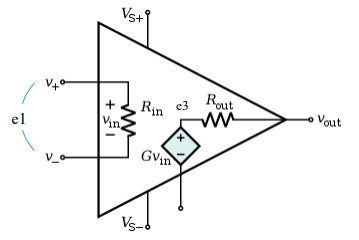
\includegraphics[width=8cm]{Imagenes/modelo_amp.png}
            \caption{Modelo Interno del Amplificador Operacional}
            \label{fig:modelo_amp}
        \end{figure}

        El método del amplificador desvanecido es una técnica utilizada en la medición de parámetros de ruido en circuitos electrónicos. La técnica consiste en introducir un amplificador de ganancia variable en el circuito para medir la relación señal a ruido (SNR) en diferentes niveles de ganancia. El proceso comienza con una señal de entrada de amplitud conocida y se varía la ganancia del amplificador para obtener diferentes niveles de amplificación. Luego, se mide la amplitud de la señal de salida y se calcula el SNR en cada nivel de ganancia. A partir de estas mediciones, se puede determinar el punto de ganancia óptimo para maximizar el SNR. El método del amplificador desvanecido se utiliza comúnmente en la caracterización de amplificadores de bajo ruido y se ha utilizado en aplicaciones como la radioastronomía, la comunicación por satélite y la medicina. 
        
        En la práctica de laboratorio usamos este método de la siguiente manera: 

        \begin{gather}
            A_v=\dfrac{V_o}{V_i}=X_{i0}+\dfrac{X_{30}AX_{i1}}{1-X_{31}A}
        \end{gather}

        Donde,

        \begin{itemize}
            \item $\mathbf{X_{i0}}$ es la Ganancia entre la entrada y salida con el amplificador desvanecido.

            \item  $\mathbf{X_{30}}$ es la ganancia entre la salida del sistema y la salida del amplificador desvanecido, con la entra del sistema apagada.

            \item  $\mathbf{X_{31}}$ es la ganancia entre la entrada del sistema y la entrada de amplificador base con el amplificador desvanecido.

            \item  $\mathbf{X_{i1}}$ es la ganancia entre la salida del amplificador base y de su entrada con $V_i= 0$.

            \item  \textbf{A} es la ganancia del amplificador base.

        \end{itemize}

    \subsection{Teorema de Blackman}

        El teorema de Blackman establece que, en un amplificador operacional realimentado, la impedancia de entrada del circuito es igual a la impedancia de entrada del amplificador operacional dividida por el factor de lazo de realimentación. Este teorema es útil para calcular la impedancia de entrada de un amplificador operacional realimentado. 
        
        El teorema de Blackman se puede expresar matemáticamente como:

        \begin{gather}
            Z_{in}=\dfrac{Z_{in_{OPAMP}}}{1+A\beta}
        \end{gather}

        Donde $Z_{in}$ es la impedancia de entrada del circuito realimentado, $Z_{in}$ del amplificador operacional es la impedancia de entrada del amplificador operacional sin realimentación, $A$ es la ganancia en lazo abierto del amplificador operacional y $\beta$ es el factor de realimentación. El teorema de Blackman se utiliza comúnmente en el diseño de circuitos con amplificadores operacionales para calcular la impedancia de entrada del circuito y garantizar que la impedancia de entrada sea lo suficientemente alta como para no afectar la señal de entrada. 
        
        En la práctica analizamos el teorema de Blackman de la siguiente manera:

        \begin{gather}
            Z_a=Z_{aa}' \, \dfrac{1-X_{31CC}A}{1-X_{31CA}A}
        \end{gather}

        Donde,

        \begin{itemize}
            \item $\mathbf{Z_{aa}'}$ la impedancia vista desde a fuente de prueba con el amplificador desvanecido.

            \item $\mathbf{X_{31CC}}$ es la ganancia desde la salida del amplificador base hasta su entrada con $V_o=0$.

            \item $\mathbf{X_{31CA}}$ es la ganancia desde la salida del amplificador base hasta su entrada con $I_a=0$
        \end{itemize}

    \subsection{Función de transferencia}

        En un amplificador operacional es la relación entre la señal de salida y la señal de entrada del amplificador, en función de la frecuencia. Esta función es importante en el diseño y análisis de circuitos amplificadores.

    \subsection{Filtros}

        Los filtros en electrónica son circuitos que se utilizan para seleccionar o rechazar ciertas frecuencias de una señal eléctrica. Los filtros pueden ser pasivos, que utilizan solo componentes pasivos como resistencias, capacitores e inductores, o activos, que utilizan componentes activos como amplificadores operacionales. Los filtros se utilizan en una amplia variedad de aplicaciones, como en la radio, la televisión, la telefonía, la música, la medicina y la investigación científica.

    \subsection{Filtros Activos}

        Los filtros activos son circuitos que incluyen uno o más amplificadores operacionales para implementar la función de filtrado. Estos filtros se utilizan para lograr un alto grado de selectividad en la respuesta en frecuencia, una mayor ganancia y una impedancia de entrada y salida más alta que los filtros pasivos. Los filtros activos se dividen en dos categorías: filtros de retroalimentación y filtros Sallen-Key. Los filtros de retroalimentación se basan en la retroalimentación de la señal de salida al amplificador operacional para lograr la función de filtrado. Los filtros Sallen-Key utilizan un par de resistencias y capacitores para lograr la función de filtrado.

        \subsubsection{Filtros Pasa Bajos}

            \begin{figure}[H]
                \centering
                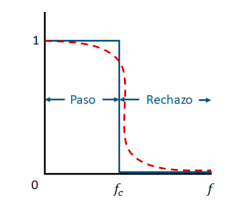
\includegraphics[width=5cm]{Imagenes/pasa_bajo.png}
                \caption{Respuesta en Frecuencia de un Filtro Pasa Bajos}
                \label{fig:pasa_bajo}
            \end{figure}
            
            En un amplificador operacional es un circuito que permite el paso de señales de baja frecuencia mientras atenúa las señales de alta frecuencia. Este tipo de filtro se utiliza comúnmente en aplicaciones de procesamiento de señales y comunicaciones. 
            
            Su función de transferencia se puede encontrar de la siguiente forma:

            \begin{gather}
                H(S)=\dfrac{H_ow_o^2}{S^2+2\zeta w_oS+w_o^2}
            \end{gather}

       \subsubsection{Filtros Pasa Banda}

            \begin{figure}[H]
                \centering
                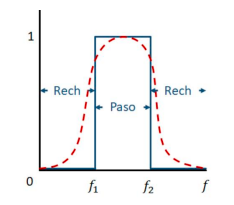
\includegraphics[width=5cm]{Imagenes/pasa_banda.png}
                \caption{Respuesta en Frecuencia de un Filtro Pasa Banda}
                \label{fig:pasa_banda}
            \end{figure} 

            En un amplificador operacional es un circuito que permite el paso de señales dentro de un rango específico de frecuencias mientras atenúa las señales fuera de ese rango. Este tipo de filtro se utiliza comúnmente en aplicaciones de procesamiento de señales y comunicaciones. Su función de transferencia se puede encontrar de la siguiente forma:

            
            \begin{gather}
                H(S)=\dfrac{H_ow_oS}{S^2+2\zeta w_oS+w_o^2}
            \end{gather}

        \subsubsection{Filtros Pasa Alta}

            \begin{figure}[H]
                \centering
                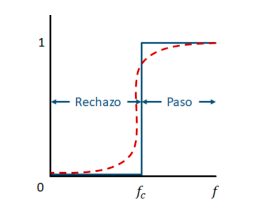
\includegraphics[width=5cm]{Imagenes/pasa_alta.png}
                \caption{Respuesta en Frecuencia de un Filtro Pasa Alta}
                \label{fig:pasa_alta}
            \end{figure} 

            En un amplificador operacional es un circuito que permite el paso de señales de alta frecuencia mientras atenúa las señales de baja frecuencia. Este tipo de filtro se utiliza comúnmente en aplicaciones de procesamiento de señales y comunicaciones. 
            
            Su función de transferencia se puede encontrar de la siguiente forma:

            \begin{gather}
                H(S)=\dfrac{H_oS^2}{S^2+2\zeta w_oS+w_o^2}
            \end{gather}

         \subsubsection{Filtros Elimina Banda}

            \begin{figure}[H]
                \centering
                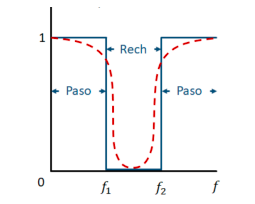
\includegraphics[width=5cm]{Imagenes/elimina_banda.png}
                \caption{Respuesta en Frecuencia de un Filtro Elimina Banda}
                \label{fig:elimina_banda}
            \end{figure} 

            En un amplificador operacional es un circuito que atenúa las señales dentro de un rango específico de frecuencias, mientras que permite el paso de señales fuera de ese rango. Este tipo de filtro se utiliza comúnmente en aplicaciones de procesamiento de señales y comunicaciones. 
            
            Su función de transferencia se puede encontrar de la siguiente forma:

            \begin{gather}
                H(S)=\dfrac{H_o(S^2+w_o^2}{S^2+2\zeta w_oS+w_o^2}
            \end{gather}

    \subsection{Retroalimentación Múltiple}

        \begin{figure}[H]
              \centering
              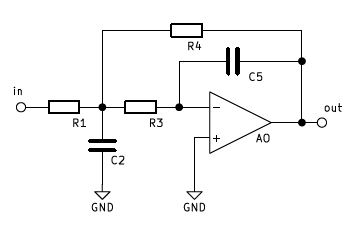
\includegraphics[width=8cm]{Imagenes/retro_multiples.png}
              \caption{Filtro Pasa Bajos con Topologías de Retroalimentaciones Múltiples}
              \label{fig:retro_multiples0}
        \end{figure}

        La retroalimentación múltiple en un amplificador operacional se refiere a una técnica de diseño que utiliza varias redes de retroalimentación para mejorar el desempeño y la estabilidad del amplificador. En esta técnica, se utilizan múltiples redes de retroalimentación para controlar la ganancia y la respuesta en frecuencia del amplificador operacional. La retroalimentación múltiple se utiliza en amplificadores operacionales de alta ganancia para mejorar la linealidad, reducir la distorsión y mejorar la respuesta en frecuencia. La técnica también se utiliza en amplificadores de potencia para mejorar la estabilidad y reducir la distorsión en altas frecuencias. En la literatura técnica, se pueden encontrar varios ejemplos de amplificadores operacionales que utilizan retroalimentación múltiple, como el amplificador operacional LM3875 de National Semiconductor y el amplificador operacional AD797 de Analog Devices

    \subsection{Filtro con Topologías Sallen-Key}

        \begin{figure}[H]
              \centering
              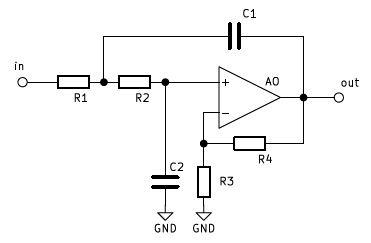
\includegraphics[width=8cm]{Imagenes/sallen_key.png}
              \caption{Filtro con Topologías Sallen-Key}
              \label{fig:sallen_key0}
        \end{figure}

        Es un tipo de filtro activo que utiliza un amplificador operacional para proporcionar ganancia y control de frecuencia en un circuito de filtro pasa bajo o pasa alto. También se conoce como filtro controlado por fuente de tensión debido al uso de un circuito RC en serie con una fuente de tensión de control para establecer la frecuencia de corte del filtro.

    \subsection{Filtro de Variables de Estado}

        \begin{figure}[H]
              \centering
              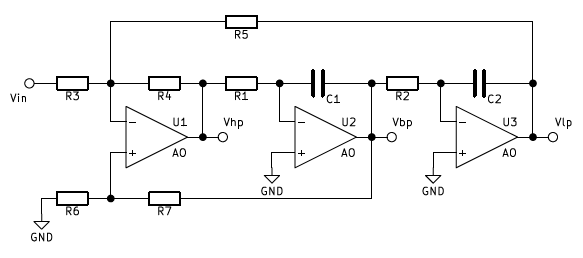
\includegraphics[width=12cm]{Imagenes/var_estado.png}
              \caption{Filtro de Variables de Estado}
              \label{fig:var_estado0}
        \end{figure}

        En el contexto de los amplificadores operacionales, una variable de estado es una magnitud que describe el estado actual del amplificador, como la tensión de entrada, la corriente de salida o la carga en un capacitor. El seguimiento de estas variables de estado es esencial en el diseño y análisis de circuitos amplificadores.

    \subsection{Fuentes de Alimentación Lineales}

        Son dispositivos electrónicos que transforman la energía eléctrica de una fuente de alimentación en una tensión continua regulada y estabilizada. Estas fuentes utilizan componentes pasivos, como resistencias y capacitores, para filtrar y regular la tensión de salida.

    \subsection{Reguladores de Tensión Monolíticos}

        Son dispositivos electrónicos que se utilizan para regular y estabilizar la tensión de salida en un circuito eléctrico. Estos reguladores se fabrican en un solo chip, lo que los hace más compactos y fáciles de usar en comparación con los reguladores de tensión discretos.

    \subsection{Error Porcentual}

    Porcentaje de error (\% de error), también conocido como porcentaje de error, es una medida de cuánto un valor difiere del valor esperado. Puede usarse para determinar qué tan lejos está un valor esperado de otro valor, pero a menudo se usa en el contexto de experimentos científicos.
    
    Se puede expresar en la siguiente ecuación:
    
    \begin{gather}
        E_r =\dfrac{|Valor_{experimental}-Valor_{teorico}|}{Valor_{teorico}} \cdot  100
        \label{eqn:error}
    \end{gather}
                 

\newpage
